\documentclass[reqno]{amsart}
\usepackage{amscd, amssymb, amsmath, amsthm}
\usepackage{graphicx}
\usepackage[colorlinks=true,linkcolor=blue]{hyperref}
\usepackage[utf8]{inputenc}
\usepackage[T1]{fontenc}
\usepackage{textcomp}
\usepackage{babel}
%% for identity function 1:
\usepackage{bbm}
%%For category theory diagrams:
\usepackage{tikz-cd}

\usepackage[backend=biber]{biblatex}
\addbibresource{notes.bib}

\setlength\parindent{0pt}

\pdfsuppresswarningpagegroup=1

\newtheorem{theorem}{Theorem}[section]
\newtheorem{lemma}[theorem]{Lemma}
\newtheorem{proposition}[theorem]{Proposition}
\newtheorem{corollary}[theorem]{Corollary}
\newtheorem{conjecture}[theorem]{Conjecture}

\theoremstyle{definition}
\newtheorem{definition}[theorem]{Definition}
\newtheorem{example}[theorem]{Example}
\newtheorem{exercise}[theorem]{Exercise}
\newtheorem{problem}[theorem]{Problem}
\newtheorem{question}[theorem]{Question}

\theoremstyle{remark}
\newtheorem*{remark}{Remark}
\newtheorem*{note}{Note}
\newtheorem*{solution}{Solution}
\newtheorem*{slogan}{Slogan}



%Inequalities
\newcommand{\cycsum}{\sum_{\mathrm{cyc}}}
\newcommand{\symsum}{\sum_{\mathrm{sym}}}
\newcommand{\cycprod}{\prod_{\mathrm{cyc}}}
\newcommand{\symprod}{\prod_{\mathrm{sym}}}

%Linear Algebra

\DeclareMathOperator{\Span}{span}
\DeclareMathOperator{\im}{im}
\DeclareMathOperator{\diag}{diag}
\DeclareMathOperator{\Ker}{Ker}
\DeclareMathOperator{\ob}{ob}
\DeclareMathOperator{\Hom}{Hom}
\DeclareMathOperator{\Mor}{Mor}
\DeclareMathOperator{\sk}{sk}
\DeclareMathOperator{\Vect}{Vect}
\DeclareMathOperator{\Set}{Set}
\DeclareMathOperator{\Group}{Group}
\DeclareMathOperator{\Ring}{Ring}
\DeclareMathOperator{\Ab}{Ab}
\DeclareMathOperator{\Top}{Top}
\DeclareMathOperator{\hTop}{hTop}
\DeclareMathOperator{\Htpy}{Htpy}
\DeclareMathOperator{\Cat}{Cat}
\DeclareMathOperator{\CAT}{CAT}
\DeclareMathOperator{\Cone}{Cone}
\DeclareMathOperator{\dom}{dom}
\DeclareMathOperator{\cod}{cod}
\DeclareMathOperator{\Aut}{Aut}
\DeclareMathOperator{\Mat}{Mat}
\DeclareMathOperator{\Fin}{Fin}
\DeclareMathOperator{\rel}{rel}
\DeclareMathOperator{\Int}{int}
\DeclareMathOperator{\sgn}{sgn}
\DeclareMathOperator{\Homeo}{Homeo}
\DeclareMathOperator{\SHomeo}{SHomeo}
\DeclareMathOperator{\PSL}{PSL}
\DeclareMathOperator{\Bil}{Bil}
\DeclareMathOperator{\Sym}{Sym}
\DeclareMathOperator{\Skew}{Skew}
\DeclareMathOperator{\Alt}{Alt}
\DeclareMathOperator{\Quad}{Quad}
\DeclareMathOperator{\Sin}{Sin}
\DeclareMathOperator{\Supp}{Supp}
\DeclareMathOperator{\Char}{char}
\DeclareMathOperator{\Teich}{Teich}
\DeclareMathOperator{\GL}{GL}
\DeclareMathOperator{\tr}{tr}
\DeclareMathOperator{\codim}{codim}
\DeclareMathOperator{\coker}{coker}
\DeclareMathOperator{\Diff}{Diff}
\DeclareMathOperator{\Bun}{Bun}
\DeclareMathOperator{\Sm}{Sm}
\DeclareMathOperator{\Fr}{Fr}
\DeclareMathOperator{\Cob}{Cob}





%Row operations
\newcommand{\elem}[1]{% elementary operations
\xrightarrow{\substack{#1}}%
}

\newcommand{\lelem}[1]{% elementary operations (left alignment)
\xrightarrow{\begin{subarray}{l}#1\end{subarray}}%
}

%SS
\DeclareMathOperator{\supp}{supp}
\DeclareMathOperator{\Var}{Var}

%NT
\DeclareMathOperator{\ord}{ord}

%Alg
\DeclareMathOperator{\Rad}{Rad}
\DeclareMathOperator{\Jac}{Jac}

%Misc
\newcommand{\SL}{{\mathrm{SL}}}
\newcommand{\mobgp}{{\mathrm{PSL}_2(\mathbb{C})}}
\newcommand{\id}{{\mathrm{id}}}
\newcommand{\MCG}{{\mathrm{MCG}}}
\newcommand{\PMCG}{{\mathrm{PMCG}}}
\newcommand{\SMCG}{{\mathrm{SMCG}}}
\newcommand{\ud}{{\mathrm{d}}}
\newcommand{\Vol}{{\mathrm{Vol}}}
\newcommand{\Area}{{\mathrm{Area}}}
\newcommand{\diam}{{\mathrm{diam}}}
\newcommand{\End}{{\mathrm{End}}}


\newcommand{\reg}{{\mathtt{reg}}}
\newcommand{\geo}{{\mathtt{geo}}}

\newcommand{\tori}{{\mathcal{T}}}
\newcommand{\cpn}{{\mathtt{c}}}
\newcommand{\pat}{{\mathtt{p}}}

\let\Cap\undefined
\newcommand{\Cap}{{\mathcal{C}}ap}
\newcommand{\Push}{{\mathcal{P}}ush}
\newcommand{\Forget}{{\mathcal{F}}orget}

\tikzset{
    labl/.style={anchor=south, rotate=135, inner sep=.5mm}
}

\title{Geometric Topology}
\author{Jonas Trepiakas}
\date{}


\begin{document}
\maketitle

\tableofcontents



\section{Continuous maps}


    \begin{definition}[]
        For a continuous map $f \colon M \to N$ between 
        topological manifolds,
        \begin{itemize}
            \item $f$ is called
                an immersion if
                locally at each point of $M$,
                it is of the form
                $\mathbb{R}^{m} \to \mathbb{R}^{n}$ 
                sending $x \mapsto \left( x,0 \right) $.
            \item $f$ is an embedding if it is
                an immersion, injective and induces a homeomorphism
                with
                its image.
            \item $f$ is a submersion if it is locally
                of the form to
                $\left( x,y \right) \mapsto x$.
        \end{itemize}
    \end{definition}

    \begin{definition}[Bundle as defined by
        Robert (is this supposed to be a fiber bundle?)]
        If 
        $f \colon M \to N$ is a continuous
        map between topological manifolds, then
        $f$ is called a bundle if it is locally
        on $N$ of the form
        $X \times V \stackrel{\pi_2}{\to } V$.
        That is, there
        exist charts, in which
        $f$ takes the form of a projection.
    \end{definition}




    \section{Bundles}

    \subsection{Fibre Bundle Theory}
    I will define things slightly differently.

    \begin{definition}[Bundle]
        A bundle is simply a triple
        $\left( E, p ,B \right) $ where
        $p \colon E \to B$ is a map.


        The pullback
        \begin{equation*}
        \begin{tikzcd}
            x^{*} E \ar[r] \ar[d]
            \ar[dr, phantom, "\lrcorner", very
            near start] & E \ar[d] \\
            x \ar[r] & B
        \end{tikzcd}
        \end{equation*}
        is called the fiber over $x$.
    \end{definition}

    \begin{definition}[Fiber bundle]
        A fiber bundle over $B$ with standard fibre
        $F$ is a bundle over $B$ such that, given
        any $x \colon 1 \to B$, the pullback of $E$ along
        $x$ is isomorphic to $F$: $x^{*}E \cong F$.
    \end{definition}

    \begin{definition}[Locally trivial fibre bundle]
        If $C$ is a site (???), then a locally trivial fibre
        bundle over $B$ with typical fibre $F$ is a bundle
        over $B$ with a cover 
        $\left( j_{\alpha} \colon U_{\alpha}
        \to B\right)_{\alpha}$ such that, for each
        index $\alpha$, the pullback $E_{\alpha}$ of
        $E$ along $j_{\alpha}$ is isomorphic in the slice
        category $C / U_{\alpha}$ to the trivial bundle
        $U_{\alpha} \times F$.
    \end{definition}




    \newpage

    \begin{definition}[Morphisms of bundles]
        Let $\left( E,p,B \right) $ and
        $\left( E',p',B' \right) $ be two bundles.
        A bundle morphism
        $\left( u,f \right) \colon
        \left( E,p,B \right) \to \left( E',p',B' \right) $ 
        is a pair of maps
        $u \colon E \to E'$ and
        $f \colon B \to B'$ such that
        \begin{equation*}
        \begin{tikzcd}
            E \ar[r, "u"] \ar[d, "p"'] & E' \ar[d, "p'"]\\
            B \ar[r, "f"'] & B'
        \end{tikzcd}
        \end{equation*}
        commutes.
    \end{definition}


    \begin{lemma}[]
        Bundles together with bundle morphisms form a category,
        which we denote $\Bun$
    \end{lemma}

    \begin{proof}
    Composition of two morphisms
    $\left( u,f \right) $ and
    $\left( u',f' \right) $ is simply done component-wise:
    $\left( u',f' \right) \circ
    \left( u,f \right) =
    \left( u' \circ u, f' \circ f \right) $.
    Now, clearly for a bundle $\left( E,p,B \right) $, we have that
    $\left( \id_E, \id_B \right) $ forms an identity morphism, and
    associativity is inherited from associativity of
    morphism composition of the ambient category.






    \end{proof}


    \begin{definition}[Slice category]
        For a category $C$ and an object
        $c \in C$, we form the category
        $c / C$ whose objects are morphisms
        $f \colon c \to x$ with domain
        $c$ and in which a morphism from
        $f \colon c \to x$ to $g \colon c\to y$ is a
        map $h \colon x\to y$ such that
        \begin{equation*}
        \begin{tikzcd}
            & c \ar[dl, "f"'] \ar[dr, "g"] &\\
            x \ar[rr, "h"'] & & y
        \end{tikzcd}
        \end{equation*}
        commutes.
        Likewise, there is a category
        $C / c$ whose objects are morphisms
        $f \colon x \to c$ with codomain $c$, and
        where a morphism from $f \colon x\to c$ to
        $g \colon y \to c$ is a map
        $h \colon x\to y$ such that
        \begin{equation*}
        \begin{tikzcd}
            x \ar[rr, "h"] \ar[dr, "f"'] && y \ar[dl, "g"]\\
                                        & c&
        \end{tikzcd}
        \end{equation*}
        commutes.\\
        The categories 
        $c / C$ and $C / c$ are called the 
        \textbf{slice categories} of $C$ 
        \textbf{under} and \textbf{over} $c$, respectively.
    \end{definition}
    
    \begin{proposition}[\cite{Riehl}]
        If $C$ is complete and cocomplete, then so
        are the slice categories
        $c / C$ and $C / c$ for any $c \in C$.
    \end{proposition}

    So in particular, we have that since
    $\Top$ is complete and cocomplete, so
    is $\Top /X$ for any $X \in \Top$.
    So the product
    $E \times_X E'$ exists in $\Top / X$ for any
    $\left[ E \to X \right] ,
    \left[ E' \to X \right] \in \Top /X$.


    \begin{definition}[$\Bun(N)$]
        For an object $N$ in the category
        $C$, we let
        $\Bun(N)$ be the slice category
        $C / N$.
    \end{definition}



    \begin{definition}[Topological and
        smooth fiber bundles with structure group]
    Let $K$ be a topological group acting on a
    Hausdorff space $F$ as a group of homeomorphisms.
    Let $X$ and $B$ be Hausdorff spaces. By a
    \textit{fiber bundle} over a base space
    $B$ with total space $X$, fiber $F$ and structure
    group $K$, we mean a bundle map
    $p \colon X \to B$ together with a maximal
    chart atlas
    $\Phi$ over $B$. Explicitly, $\Phi$ is a collection
    of trivializations
    $\varphi  \colon U
    \times F \to p^{-1}(U)$ such that
    \begin{enumerate}
        \item each point of $B$ has a neighborhood
            over which there is a chart in
            $\Phi$
        \item if $ \varphi \colon U \times F
            \to p^{-1} (U) $ is in
            $\Phi$ and  $V \subset U$, then the
            restriction
            $\varphi |_{V \times F}$ is also in
            $\Phi$.
        \item If $\varphi , \psi  \in \Phi$ are
            charts over $U$ then there exists a map
            $\theta \colon U \to K$ such that
            $\psi \left( u, y \right)
            = \varphi \left( u, \theta(u) (y) \right) $
        \item the set $\Phi$ is maximal among the collections
            satisfying the (1),(2) and (3)
    \end{enumerate}
    The fiber bundle is called smooth if all the spaces
    are smooth manifolds and all maps involved are smooth.
\end{definition}

\begin{example}{The product bundle}
    If we have a space $B = X \times Y$ and let
    $p \colon B \to X$ be the projection
    $p(x,y) = x$, then seeing as
     $p^{-1}(X) = X\times Y$, we automatically obtain
     an trivialization
      $\varphi  \colon p^{-1}(X) \cong X \times Y$.
      The sections (aka cross sections) of 
      $B$, i.e., continuous maps
      $X \to X \times Y$ is then just simply equivalent to
      graphs of maps $X \to Y$. The fibres are
      all homeomorphic.
      Since a single trivialization works for all
      of $X$, this exhibits $X \times Y$ 
      as a fiber bundle over $X$ with trivial structure group.
\end{example}

\begin{example}[Möbius band]
    Take the base space $X = S^{1}$ obtained from
    $I$ by identifying ends. Let $Y = I$ be the fibre.
    We can obtain the Möbius bundle from
    $I \times I$ by matching the ends by a twist. This
    descends to a projection
    $p \colon B \to S^{1} = X$ where $B$ is the Möbius band.
    There are many cross-sections: any curve
    $I \to I \times I$ by $t \mapsto \left( t, 
    \gamma(t) \right) $ for some $\gamma \colon I \to I$ 
    such that $\gamma(0) = 1- \gamma(1)$ works. In particular,
    any two cross-sections agree on at least one point (see
    picture \cite[p. 4]{Steenrod}. The structure group
    is $\mathbb{Z} /2$.
\end{example}

\begin{example}[Klein Bottle]
    The Klein bottle can be obtained similarly, choosing
    $I$ as the fibre but $S^{1}$ as the base space and then
    quotienting the ends of $S^{1} \times I$. Again, see
    \cite[p. 4]{Steenrod}.
\end{example}

\begin{example}[Covering Spaces]
    A covering space $B$ of a space $X$ is another example
    of a bundle. The projection
    $p \colon B \to X$ is the covering map.
    In particular, a covering space is a
    locally trivial fibre bundle where the fibre is a discrete
    space.\\
\end{example}

\subsubsection{Coordinate bundles and fibre bundles}

\begin{definition}[Transformation groups]
    Recall that if $G$ is a topological group and
    $Y$ is a topological space, we say that
    $G$ is a topological transformation group of $Y$ relative
    to a map $\eta \colon G \times Y \to Y$ if
    \begin{enumerate}
        \item $\eta$ is continuous
        \item $\eta (e,-) = \id$ 
        \item $\eta \left( g_1g_2,y \right) 
            = \eta \left( g_1, \eta(g_2,y) \right) $.
    \end{enumerate}
    We shall often implicitly assume $\eta$ as given and
    abbreviate $\eta (g,y)$ by $g\cdot y$, so that the above
    become that $\cdot $ is continuous,
    $e\cdot y =y$ for all $y$ and
    $\left( g_1g_2 \right) \cdot y = g_1\cdot \left( g_2\cdot y
    \right) $.
\end{definition}

\begin{definition}[Effective action]
    We say that $G$ is effective if
    $g \cdot y = y$ for all $y$ implies that
    $g = e$.
\end{definition}

\begin{definition}[Coordinate Bundle]
    A coordinate bundle
    $\mathcal{B}$ is a collection as follows:
    \begin{enumerate}
        \item A bundle space $B$ 
        \item a base space $X$ 
        \item a projection $p \colon B \to X$ 
        \item a space $Y $ called the fibre
        \item an effective topological transformation group
            $G$ acting on $Y$, called the
            (structure) group of the bundle
        \item A family $\left\{ V_\alpha \right\} $ of open
            sets covering $X$ called coordinate neighborhoods
        \item trivializations $\varphi_\alpha$ 
            giving homeomorphisms
            \[
            \varphi_a \colon V_a \times Y \to p^{-1}(V_a)
            \] 
            called coordinate functions.
    \end{enumerate}
    restricted to the following requirements
    \begin{enumerate}
        \item 
        \begin{equation*}
        \begin{tikzcd}
            V_{\alpha} \times Y \ar[rr, "\varphi_{\alpha}"]
            \ar[dr, "\pi_1"']
            && p^{-1}(V_{\alpha})
            \ar[dl, "p"] \\
                                        & V_{\alpha}&
        \end{tikzcd}
        \end{equation*}
        commutes.
    \item letting the map
        $\varphi_{j,x} \colon Y \to p^{-1}(x)$ be defined
        by
        \[
        \varphi_{j,x}(y) = \varphi_j (x,y)
        \] 
        then for each $x \in V_{\alpha} \cap V_{\beta}$,
        $\varphi_{j,x}^{-1}\varphi_{i,x} (-) \colon
        Y \to Y $ is the same as
        $g \cdot (-) \colon Y \to Y$ for some
        $g \in G$.
    \item the map $g_{\alpha \beta} \colon V_\alpha
        \cap V_\beta \to G$ by
        $g_{\alpha \beta}(x) = 
        \varphi_{\alpha,x}^{-1} \varphi_{\beta,x}$ is continuous.
    \end{enumerate}
\end{definition}

And immediate consequence of the definition is that
\[
g_{\gamma \beta} (x) g_{\beta \alpha}(x) = 
g_{\gamma \alpha}(x), \quad x \in V_{\alpha} \cap V_{\beta}
\cap V_{\gamma}.
\] 
It is also convenient to introduce the map
$p_{\alpha} \colon p^{-1}(V_{\alpha}) \to Y$ given by
$p_{\alpha}(b) = \varphi_{\alpha,p(b)}^{-1}(b)$.

We obtain the identities
\begin{align*}
    p_\alpha \varphi_\alpha (x,y) &= y\\
    \varphi_\alpha \left( p(b), p_\alpha(b) \right) &= b\\
    g_{\alpha \beta}\left( p(b) \right) \cdot 
    p_\beta(b) = p_\alpha(b)
\end{align*}

\begin{definition}[Fibre bundle in terms of coordinate bundles]
    Two coordinate bundles
    $\mathcal{B}$ and $\mathcal{B}'$ are
    equivalent in the strict sense i they
    have the same bundle space, base space, projection,
    fibre and structure group and their coordinate functions
    satisfy that
    \[
    \overline{g}_{kj} = \varphi_{k,x}'^{-1} \varphi_{j,x}
    \] 
    coincide with the operation of an element of $G$ and the
    map
    $\overline{g}_{kj} \colon
    V_j \cap V_{k}' \to G$ is continuous.

    Then a fibre bundle is a maximal coordinate bundle
    with respect to this equivalence relation.
\end{definition}

\begin{definition}[Mappings of fibre bundles]
    Let $\mathcal{B}$ and $\mathcal{B}'$ be two
    coordinate bundles having the same fibre and structure group.
    A map $h \colon \mathcal{B} \to \mathcal{B}'$ 
    is a tuple 
    $\left( h, \overline{h} \right) $ with
    $h \colon B \to B'$ and $\overline{h} \colon X \to X'$ 
    such that
    \begin{equation*}
    \begin{tikzcd}
        B \ar[d] \ar[r, "h"] & B' \ar[d] \\
        X \ar[r, "\overline{h}"] & X'
    \end{tikzcd}
    \end{equation*}
    commutes and
    \[
    \overline{g}_{\alpha \beta}(x) = 
    \varphi_{\alpha, x'}'^{-1} h_x \varphi_{\beta ,x} =
    p_k' h_x \varphi_{\beta, x}
    \] 
    coincides with the operation of some $g \in G$ on
    $Y$. Here $h_x \colon Y_x \to Y_{x'}$ is the map
    $h(x,-)$, where $x' = \overline{h}(x)$.
    Furthermore, the map
    \[
    \overline{g}_{\alpha \beta}\colon
    V_{\beta} \cap \overline{h}^{-1}\left( V_{\alpha}' \right) 
    \to G
    \] is assumed to be continuous.
\end{definition}

In particular, since
$\overline{g}_{\alpha \beta}(x)$ acts by
some $g \in G$ on $Y$ which is through homeomorphisms,
we obtain that since
$\varphi_{\alpha,x'}'^{-1}$ and
$\varphi_{\beta, x}$ are also homeomorphisms,
$h_x$ is a homeomorphism of the fibres.

The mapping transformations $\overline{g}_{\alpha \beta}$ satisfy
\begin{align*} \label{eq:Omega}\tag{$\Omega$}
    \overline{g}_{\alpha \beta}(x) g_{\beta \gamma}(x)
    &= \overline{g}_{\alpha \gamma}(x)\\
    g_{\alpha \beta}' \left( \overline{h}(x) \right) 
    \overline{g}_{\beta \gamma}(x) &= \overline{g}_{\alpha \gamma}
    (x).
\end{align*}

\begin{lemma}[]
    Let $\mathcal{B}, \mathcal{B}'$ be coordinate bundles having
    the same fibre $Y$ and group  $G$, and let
    $\overline{h} \colon X \to X'$ be a map of one
    base space into the other. Let
    $\overline{g}_{kj} \colon
    V_j \cap \overline{h}^{-1}(V_k') \to G$ be a set
    of continuous maps satisfying \eqref{eq:Omega}. Then
    there exists a unique fibre bundle map
    $h \colon \mathcal{B} \to \mathcal{B}'$ inducing
    $\overline{h}$ and having
    $\left\{ \overline{g}_{jk} \right\} $ as its
    mapping transformations.
\end{lemma}

\begin{lemma}[]
    Let $\mathcal{B}, \mathcal{B}'$ be coordinate bundles having
    the same fibre and group, and let $h \colon \mathcal{B}
    \to \mathcal{B}'$ be a bundle map such that
    the induced map $\overline{h} \colon X \to X'$ is
    a homeomorphism. Then
    $h$ has a continuous inverse
    $h^{-1} \colon B' \to B$, and
    $h^{-1}$ is a bundle map
    $\mathcal{B}' \to \mathcal{B}$.
\end{lemma}


\begin{definition}[]
    Two coordinate bundles 
    $\mathcal{B}$ and $\mathcal{B}'$ with the same
    base space, fibre and group are said to be
    equivalent if there exists a fibre bundle
    map $\mathcal{B}\to \mathcal{B}'$ which induces the
    identity of the common base space.\\
    Two fibre bundles having the same base space,
    fibre and group are said to be equivalent if they
    have representative coordinate bundles which are
    equivalent.
\end{definition}

\begin{lemma}[]\label{bundle-equiv-in-terms-of-maps}
    Let $\mathcal{B},\mathcal{B}'$ be coordinate bundles
    having the space base space, fibre and group. Then
    they are equivalent if and only if
    there exist continuous maps
    \[
    \overline{g}_{kj} \colon V_j \cap V_{k}' \to G
    \] 
    such that
    \begin{align*}
        \overline{g}_{ki}(x) 
        &= \overline{g}_{kj}(x) g_{ji}(x)\\
        \overline{g}_{lj}(x) 
        &= g_{lk}'(x) \overline{g}_{kj}(x)
    \end{align*}.
\end{lemma}

\begin{lemma}[]
    Let $\mathcal{B},\mathcal{B}'$ be two coordinate bundles
    with the same base space, fibre, group and coordinate
    neighborhoods. Let
    $g_{ji}, g_{ji}'$ denote their coordinate transformations.
    Then $\mathcal{B}, \mathcal{B}'$ are equivalent
    if and only if there exist continuous functions
    $\lambda_j \colon V_j \to G$ such that
    \[
    g_{ji}'(x) = \lambda_j(x)^{-1} g_{ji}(x)
    \lambda_i(x).
    \] 
\end{lemma}

\begin{lemma}[]
    Let $\mathcal{B}, \mathcal{B}'$ be coordinate bundles
    having the same fibre and group, and let
    $h \colon \mathcal{B} \to \mathcal{B}'$ be a fibre
    bundle map. Corresponding to each
    section $f' \colon X' \to B'$, there
    exists a unique section
    $f \colon X \to B$ such that
    \begin{equation*}
    \begin{tikzcd}
        B  \ar[r, "h"] & B'  \\
        X \ar[r, "\overline{h}"'] \ar[u, "f"] & X' \ar[u, "f'"']
    \end{tikzcd}
    \end{equation*}
    commutes.
    The section  $f$ is said to be induced by
    $h$ and $f'$ and will be denoted
    $h^{*}f'$.
\end{lemma}

\subsubsection{Construction of a bundle from coordinate
transformations}
\begin{definition}[]
    Let $G$ be a topological group and $X$ a space.
    By a \textit{system of coordinate transformations in
    $X$ with values in $G$} is meant an indexed covering
    $\left\{ V_j \right\} $ of $X$ by open sets and
    a collection of continuous maps
    \[
    g_{ji} \colon V_{i} \cap V_j \to G
    \] 
    such that
     \[
    g_{kj}(x) g_{ji}(x) = g_{ki}(x).
    \] 
\end{definition}

\begin{remark}[]
    We have so far seen that any bundle over
    $X$ with group $G$ determines such a set of
    coordinate transformations. We now state a converse.
\end{remark}

\begin{theorem}[Existence]\label{Existence-theorem}
    If $G$ is a topological transformation group of
    $Y$, and $\left\{ V_j \right\} , 
    \left\{ g_{ij} \right\} $ is a system
    of coordinate transformations in the space
    $X$, then there exists a bundle $\mathcal{B}$ with
    base space $X$, fibre $Y$, group $G$ and
    coordinate transformations
    $\left\{ g_{ij} \right\} $. Furthermore,
    any such bundles are equivalent.
\end{theorem}

\subsubsection{Factor/Quotient/Coset Spaces of Groups}


\begin{definition}[Local section of $G$]
     Let $G$ be a closed subgroup of $B$. Then
     $G$ is a point
     $x_0 \in B / G$. A \textit{local section}
     of $G$ in $B$ is a function $f $ mapping a neighborhood
     $V$ of $x_0$ continuously into $B$ and such that
     $p f (x) = x$ for each $x \in V$.
\end{definition}



\subsubsection{Enlarging the group of a bundle}

Let $H$ be a closed subgroup of the
topological group $G$.
If $\mathcal{B}$ is a bundle with group $H$, the
same coordinate neighborhoods, and the same
coordinate transformations, altered
only by regarding their values as belong to $G$, define
a new bundle called the
\textit{$G$-image of $\mathcal{B}$}.\\
\begin{note}
    If $H$ operates on the fibre $Y$, it may or may not
    occur that $G$ operates on $Y$ or even 
    that such operations can be defined.
\end{note}

\begin{definition}[$G$-equivalence]
    Let $H,K \le G$ be closed subgroups, and let
    $\mathcal{B},\mathcal{B}'$ be bundles having the same
    base space and structure groups
    $H,K$, respectively. We say that
    $\mathcal{B},\mathcal{B}'$ are \textit{equivalent in
    $G$} or \textit{$G$-equivalent} if the
    $G$-images of $\mathcal{B}$ and
    $\mathcal{B}'$ are equivalent.
\end{definition}


\subsubsection{The Principal Bundle and the Principal Map}

\begin{definition}[Principal $G$-bundle]
    A bundle
    $\mathcal{B} = 
    \left\{ B,p,X,Y,G \right\} $ is called
    a principal bundle if $Y = G$ and
    $G$ operates on $Y $ by left translations.
\end{definition}

\begin{definition}[Associated prinicipal bundle]
    Let $\mathcal{B} = \left\{ B,p,X,Y,G \right\} $ be
    an arbitrary bundle. The
    \textit{associated principal bundle}
    $\tilde{B}$ of $\mathcal{B}$ is the bundle given
    by the construction/existence theorem using the
    same base space, the same $\left\{ V_j \right\} $,
    the same $\left\{ g_{ji} \right\} $ and
    the same group $G$ as for $\mathcal{B}$, but
    replacing $Y$ by $G$ and allowing $G$ to operate
    on itself by left translations.
\end{definition}

\begin{theorem}[Equivalence theorem]\label{Equivalence-theorem}
    Two bundles having the same base space, fibre
    and group are equivalent if and only if their
    associated principal bundles are equivalent.
\end{theorem}

\begin{proof}
    By Lemma \ref{bundle-equiv-in-terms-of-maps}, 
    equivalence of bundles is purely a property
    of the coordinate transformations.
\end{proof}






\newpage
\begin{definition}[Manifold bundle]
    Let $M$ be a smooth manifold. A
    manifold bundle over $M$ with structure group
    $G$ is a fiber
    bundle
    $W \to E \to M$ with
    structure group $G$ such that
    $E$ is a manifold and $E \to M$ is continuous.\\
    We say a manifold bundle over $M$ is a smooth
    manifold bundle if it is
    a smooth fiber bundle as well as
    a manifold bundle and $G$ acts by diffeomorphisms
    on $M$.
\end{definition}


    \begin{definition}[Associated bundles]
        Let $M$ be a smooth manifold, and
        fix a manifold bundle
        $E \stackrel{\xi}{\to } M$ with fibre a smooth
        manifold $W$ and structure group
        $G \le \Homeo (W)$. Given another smooth manifold
        $W'$ such that there exists an injective group
        homomorphism $\iota \colon G \hookrightarrow
        \Homeo\left( W' \right) $, the associated
        $W'$-manifold bundle of $\xi$ is defined
        as follows. Let
        $\left\{ U_{\alpha}, \varphi_{\alpha} \right\}_{\alpha}$ 
        be a cover of $M$ by open neighborhoods together with
        trivializations
        $\varphi_{\alpha}$ of $\xi$. Transition maps
        $\varphi_{\alpha} \varphi_{\beta}^{-1}$ give rise
        to transition function
        $g_{\alpha \beta} \colon U_{\alpha} \cap
        U_{\beta} \to G \le \Homeo(W)$ satisfying the
        cocycle condition. We define the associated
        $W'$-manifold by gluing trivializations
        $U_{\alpha} \times W'$ along transition maps
        \[
        \iota \circ g_{\alpha\beta} \colon U_{\alpha}
        \cap U_{\beta} \to G 
        \stackrel{\iota}{\to } \Homeo\left( W' \right) .
        \] 
    \end{definition}

    \begin{definition}[Structure group reduction]
        Fix a manifold bundle
        $\xi \colon E \to M$ over a smooth manifold
        $M$, with fibre a smooth manifold $W$ and structure
        group $G$. Given a subgroup $H \le G$, $\xi$ 
        is said to admit a structure group reduction to
        $H$ if it is isomorphic to a bundle so that all transition
        maps $g_{\alpha \beta} \colon U_{\alpha} \cap
        U_{\beta} \to G$ take values in $H$.
    \end{definition}

    \begin{problem}[Change of fibres of bundles]
        Let $W_0$ and $W_1$ be two smooth manifolds, and
        let $G$ be a group which we assume as a simultaneous
        subgroup of both $\Homeo (W_0)$ and
        $\Homeo(W_1)$, i.e., we have injective group homomorphisms
        $\iota_0 \colon G \hookrightarrow
        \Homeo(W_0)$ and
        $\iota_1 \colon G \hookrightarrow (W_1)$. Given a
        fixed smooth manifold $M$, construct a bijection
        $\Bun_G^{W_0}(M) \to \Bun_G^{W_1}(M)$, where
        $\Bun_G^{W_i}(M)$ denotes the set of
        isomorphism classes of manifold bundles with fibre
        $W_i$ and structure group $G$.
    \end{problem}

    \begin{proof}
        Let
        $\mathcal{B} = \left\{ B,p,X,W_0,G \right\} 
        \in \Bun_G^{W_0}$.
        By Theorem \ref{Equivalence-theorem}, the
        bundle $\mathcal{B}$ is equivalent
        to its associated principal bundle
        $\tilde{\mathcal{B}} = 
        \left\{ B,p,X,G,G \right\} $. But by
        assumption, $G$ embeds into
        $\Homeo(W_1)$, so by Theorem 
        \ref{Existence-theorem}, also
        $\tilde{B}$ is equivalent to
        $\left\{ B,p,X,W_1,G \right\} =:
        \mathcal{B}'$ which has the
        same coordinate transformations. Thus
        $\tilde{B}$ and $\tilde{B}'$ are equivalent.
        Now, seeing as equivalence of bundles is purely determined
        by their base space, fibre, structure group and
        coordinate transformations,
        this gives an injective map
        $\Bun_G^{W_0} \to \Bun_G^{W_1}$. Seeing
        as we can do the exact same thing to obtain an
        injective map
        $\Bun_{G}^{W_1} \to \Bun_G^{W_0}$, we obtain
        a bijection by Schröder-Bernstein.
    \end{proof}

    \subsubsection{Associated bundles and relative bundles}

    \begin{definition}[]
        Two bundles, having the same base space
        $X$ and the same group $G$, are said to be
        \textit{associated} if their associated 
        principal bundles are equivalent.
    \end{definition}

    \begin{exercise}[]
        Check that the relation of being associated is
        reflexive, symmetric and transitive.
    \end{exercise}

    \begin{definition}[Relative bundle]
        Let
        $\mathcal{B} = \left\{ B,p,X,Y,G \right\} $ be
        a bundle. Let $A \subset X$ be a closed subspace and
        $H \le G$ a closed subgroup. If, for every
        $i,j$ and every $x \in V_i \cap V_j \cap A$, the
        coordinate transformation $g_{ji}(x)$ is an
        element of $H$, then the portion of the bundle
        over $A$ may be regarded as a bundle with
        group $H$. One simply restricts the coordinate
        neighborhoods and functions to $A$. Whenever
        this occurs, we say that $\mathcal{B}$ is
        a \textit{relative $\left( G,H \right) $-bundle
        over the base space $\left( X,A \right) $}.
    \end{definition}

    \begin{definition}[$(G,H)$-equivalence]
        Let $\mathcal{B}$ be a 
        $\left( G,H \right) $-bundle over
        $(X,A)$ and let
        $\mathcal{B}'$ be an 
        $\left( H,H \right) $-bundle over
        $(X,A)$. A $\left( G,H \right) $-equivalence
        of $\mathcal{B}$ and $\mathcal{B}'$ is a map
        $h \colon \mathcal{B}\to \mathcal{B}'$ which is,
        first, a $G$-equivalence of the two absolute
        bundles over $X$, and, second, an
        $H$-equivalence when restricted to the 
        portions of $\mathcal{B},\mathcal{B}'$ lying over $A$.
    \end{definition}


    \begin{slogan}
        The smaller the group of a bundle, the simpler
        the bundle.
    \end{slogan}

    \subsubsection{The canonical section of
    a relative bundle}

    Let $\mathcal{B}$ be a 
    $\left( G,H \right) $-bundle over
    $(X,A)$. Let
    $\mathcal{B}'$ denote the associated bundle over
    $X$ having $G /H$ as fibre and $G$ acting
    on the fibre by left translations.
    Let $e_0$ denote the coset
    of $H$ treated as an element of $G /H$.
    We define a section over $A$ of the bundle
    $\mathcal{B}'$ by
    \[
    f_0(x) = \varphi_j' (x,e_0), \quad x \in V_j \cap A.
    \] 
    If $x \in V_i \cap V_j \cap A$, then
    \[
    \varphi_j'(x,e_0) = 
    \varphi_i'\left( x, g_{ij}(x) \cdot e_0 \right) 
    = \varphi_i' (x, e_0)
    \] 
    since $g_{ij}(x) \in H$. Thus
    $f_0$ defines a section over $A$.
    We call $f_0$ the \textit{canonical section of the
    $(G,H)$-bundle}.



    \subsubsection{Structure Group Reduction}


    \begin{definition}[]
        For a bundle where  the fibres are
        of the form $G /H$, if
        $G$ operates effectively on
        $G /H$, we obtain an associated bundle;
        otherwise, a weakly associated bundle.
    \end{definition}

    \begin{theorem}[]
        Let $H \le G$ be a closed subgroup which
        has a local section. 
        A $\left( G,H \right) $-bundle over
        $\left( X,A \right) $ is
        $(G,H)$-equivalent to an
        $\left( H,H \right) $-bundle over
        $\left( X,A \right) $ if and only if the 
        canonical section (defined only over $A$ ) can
        be extended to a full section of the
        weakly associated bundle with fibre
        $G /H$.
    \end{theorem}

    \begin{corollary}
        If $H$ has a local section in $G$, then
        a $G$-bundle over $X$ is $G$-equivalent to an
        $H$-bundle if and only if the weakly associated
        bundle with fibre $G /H$ has a section.
    \end{corollary}


    Tomorrow, check out the link
    \url{https://math.stackexchange.com/questions/2015174/structure-group-of-tangent-bundle-of-riemannian-manifold}

    \subsubsection{Associated frame bundles and structure
    group reductions}


    \begin{problem}[]
    For a rank $d$ vector bundle
    $\xi \colon E \to M$ over a smooth manifold, we 
    define the associated frame bundle $\Fr \left( \xi \right) $ 
    as the associated $\GL_d \left( \mathbb{R} \right) $-bundle.
        \begin{enumerate}
            \item For $M$ a smooth $d$-dimensional
                manifold, we define its frame
                bundle $\Fr (M)$ as the associated
                frame bundle of its tangent bundle
                $TM$. Show that
                $\Fr(M) \to M$ is a principal 
                $\GL_d \left( \mathbb{R} \right) $-bundle.
            \item Show that a manifold is
                orientable if and only if its
                frame bundle $\Fr (M)$ admits a
                $\GL_d^{+} (\mathbb{R})$ reduction of
                its structure group, where
                $\GL_d^{+}(\mathbb{R})$ is the subgroup
                of the general linear group consisting
                of invertible matrices with positive determinant.
            \item Show that a structure bundle reduction of
                the frame bundle
                $\Fr(M)$ to the orthogonal group
                $O(n) \le \GL_d(\mathbb{R})$ corresponds
                to a choice of a bundle metric on the tangent
                bundle  $TM$ of $M$.
        \end{enumerate}
    \end{problem}


    \subsubsection{The Induced Bundle}

    \begin{definition}[First definition of the induced bundle]
        Suppose we have a bundle
        $\mathcal{B}'$ over a base
        space $X'$, fibre $Y$ and group $G$ which
        is uniquely determined up to isomorphism
        by a system of coordinate transformations
        $\left\{ V_{\alpha}' \right\} $ and
        $\left\{ g_{\alpha \beta}' \right\} $.
        Suppose now we have a map
        $\eta \colon X \to X'$.
        The \textit{induced bundle}
        $\eta^{*}\mathcal{B}'$ having base space
        $X$, fibre $Y$ and group $G$ is defined
        by pulling back the system of coordinate transformations
        by letting $\left\{ V_\alpha \right\} $ with
        $V_{\alpha} = \eta^{-1}\left( V_{\alpha}' \right) $ 
        and
        $\left\{ g_{\alpha \beta} \right\} $ with
        $g_{\alpha \beta}(x)
        = g_{\alpha \beta}' \circ \eta(x)$ be the
        system of coordinate transformations of
        $\eta^{*}\mathcal{B}'$ and then constructing a
        bundle using the Existence theorem
        (Theorem \ref{Existence-theorem}).
        We define a map
        $h \colon
        \eta^{*}\mathcal{B}' \to \mathcal{B}'$ (which,
        recall, is a map $B \to B'$ ) by
        \[
            h(b) =
        \varphi_j' \left( 
        \eta p(b), p_j(b) \right) , \qquad
    p(b) \in V_j
\]

        Recall that
        $p_j \colon
        p^{-1}(V_j) \to Y$ is given by
        $p_j(b) = \varphi_{j,p(b)}^{-1}(b) \in Y$.
        Indeed then
        $\eta p(b) \in X'$, so
        $\left( \eta p(b), p_j(b) \right) \in 
        X' \times Y$, and 
        $\varphi_j'$ is defined on some open
        subset of this space.
        To show that $h$ is well-defined, we
        must show that it agrees on overlaps.
        If $p(b) \in V_i \cap V_j$, then
        \begin{align*}
        \varphi_j'\left( \eta(p(b)), p_j(b) \right) 
        &= \varphi_i' \left( \eta(p(b)),
        g_{ij}' \left( \eta\left( p(b) \right)
    \cdot p_j(b) \right) \right) \\
        &= \varphi_i' \left( \eta (p(b)),
        g_{ij}(x) \cdot p_j(b) \right) 
        = \varphi_i' \left( \eta (p(b)),
        p_i(b) \right) 
        \end{align*}
        Furthermore, all the maps in the definition
        of $h$ are continuous, so $h$ is continuous.\\

        In particular,
        $p' h(b) = \eta(p(b))$, so
        indeed $h$ induces $\eta$ on $X \to X'$. I.e.,
        \begin{equation*}
        \begin{tikzcd}
            B \ar[r, "h"] \ar[d] & B'\ar[d] \\
            X \ar[r, "\eta"] & X'
        \end{tikzcd}
        \end{equation*}
        commutes.
        Lastly, we want to show that $h$ is a bundle map.

        This means that we must show that
        for
        $x \in V_j \cap \eta^{-1}(V_k')$, the map
        \[
        \overline{g}_{kj}(x) =
        \varphi_{k,x'}'^{-1} h_x \varphi_{j,x} = 
        p_k' h_x \varphi_{j,x} \colon Y \to Y
        \] 
        coincides with the operation of some $g \in G$
        on $Y$. That is, that 
        $\overline{g}_{kj} \colon
        V_{j} \cap V_{k} \to G$ is continuous for any
        $k,j$.
        But indeed
        \begin{align*}
            \overline{g}_{kj}(x)\cdot y
            &= \varphi_{k,x'}'^{-1} h_x \varphi_{j,x}(y)\\
            &= 
            \varphi_{k,x'}'^{-1} 
            \varphi_j' \left( x',
            p_j \left( \varphi_{j,x}(y) \right)  \right) \\
            &= \varphi_{k,x'}'^{-1} 
            \varphi_{j}' \left( x', y \right) \\
            &= \varphi_{k,x'}'^{-1} \varphi_{j,x'}'(y)\\
            &= g_{k,j}' (x') \cdot y
        \end{align*}
        so $\overline{g}_{kj} =
        g_{kj}' \circ \eta = g_{kj}$, and it is
        a continuous map of
        $V_{k} \cap V_j $ into $G$.
        
    \end{definition}



    \begin{definition}[Second definition of the induced bundle]
        Suppose $\mathcal{B}', X$ and $\eta$ are
        as before. Form the product space
        $X \times B'$ and let
        $p \colon X \times B' \to X, h\colon
        X \times B' \to B'$ be the natural projections.
        Define $B = X \times_{X'} B' :=
        \left\{ (x,b') \in X \times B'  \mid 
        \eta (x) = p'(b') \right\} $ to be the
        fibered product.\\
        We want to give
        $\left[ p \colon B \to X \right] $ a fibre
        bundle structure (by giving it a coordinate bundle structure).
        Define
        $V_j = \eta^{-1} (V_j')$ and
        set
         \[
        \varphi_j(x,y) = \left( x, 
        \varphi_j'\left( \eta(x),y \right) \right).
        \] 
        Let's give these maps some motivation.
        For these to be trivializations,
        we want
        $\varphi_j$ to be homeomorphisms
        $p^{-1}(V_j) \cap B = p|_B^{-1}\left( V_j \right) 
        \cong V_j \times Y$.
        Now,  $\varphi_j$ simply maps
        $x$ to $x$ in the first coordinate, but
        $\varphi_j'$ by assumption maps
        $V_j' \times Y$ homeomorphically onto
        $p'^{-1}(V_j')$. Hence in particular,
        $\varphi_j'\left( \eta(x), y \right) 
        \in p'^{-1}(V_j') \subset B'$. So
        $\left( x, \varphi_j' \left( \eta(x), y \right)  \right) 
        \in B$ if and only if
        $\eta (x) = p' \left( 
        \varphi_j' \left( \eta(x), y \right) \right) $, but
        this is true by assumption.
        Furthermore,
        $\left( x, \varphi_j' \left( \eta(x),y \right)  \right) 
        \in X \times B'$, so applying $p$, we get
        $p \left( x, \varphi_j' \left( \eta(x),y \right)  \right) 
        = x$ which is in
        $V_j$ when $x \in V_j$.
        Hence putting things together,
        $\varphi_j$ maps
        $V_j \times Y$ to
        $p^{-1}\left( V_j \right) \cap B$.
        We, in fact, want to show that 
        $\varphi_j$ is a homeomorphism
        of these spaces. For this, simply note that
        the map
        $\left( u,v \right) \mapsto 
         \left( u, \pi_2 \circ \varphi_j'^{-1}(v) \right) $ 
         is an inverse.\\
         Lastly, let for
         $x \in V_i \cap V_j$,
         $g_{ij}(x) = \varphi_{i,x}^{-1} \varphi_{j,x}
         = p_i \varphi_{j,x}$


         Note then that
         \begin{align*}
             g_{ij}(x) y
             &= p_i \varphi_{j,x}(y)\\
             &= p_i \left( x, \varphi_j' \left( 
             \eta (x), y\right)  \right) \\
             &= p_i' \varphi_j' \left( \eta(x), y \right) \\
             &= g_{ij}' \left( \eta(x) \right) y
         \end{align*}
 
         So the clutching functions
         are simply
         $g_{ij}' \circ \eta$ which are indeed
         continuous.

    \end{definition}

    \begin{theorem}[Equivalence
        Theorem/pullbacks of fibre bundles with the same
        fibre and group exist
        ]\label{Equivalence-Theorem-Induced-Bundles}
        Let $\mathcal{B},\mathcal{B}'$ be two bundles having
        the same fibre and group and
        $h \colon \mathcal{B} \to \mathcal{B}'$ a bundle
        map. Let
        $\eta \colon X \to X'$  be the induced map of
        base spaces. Then the induced
        bundle $\eta^{*}\mathcal{B}'$ is equivalent to
        $\mathcal{B}$, and there
        is an equivalence
        $h_0 \colon \mathcal{B} \to \eta^{*}\mathcal{B}'$ such
        that $h$ is the composite
        $h = h^{*} \circ h_0$ where
        $h^{*} \colon \eta^{*}\mathcal{B}' \to 
        \mathcal{B}'$ is the induced map:

        \begin{equation*}
        \begin{tikzcd}
            B \ar[dr, "\exists", dashed]
            \ar[drr, bend left] \ar[ddr, bend right] & & \\
              & X \times_{X'}B'
            \cong \eta^{*}B' \ar[r] \ar[d]
            \ar[dr, phantom, "\lrcorner", very near start]
              & B' \ar[d] \\
              & X \ar[r, "\eta"] & X'
        \end{tikzcd}
        \end{equation*}
    \end{theorem}

    \begin{definition}[Orientability]
        A smooth manifold
        $M$ is called \textit{orientable} if
        for all smooth maps
        $S^{1} \to M$,
        $f^{*} TM$ is trivializable.
        That is,
        $\left[ f^{*}TM \to S \right] $ is a
        trivial bundle.
    \end{definition}



    \subsection{A Bundle Theory}

    \begin{note}
        A "Bundle Theory" is also called a 
        Cartesian Fibration over
        $\Sm$.
    \end{note}

    \begin{definition}[Essential fibers]
        For a functor
        $F \colon \mathcal{B} \to \mathcal{C}$ and an object
        $M \in \mathcal{C}$, the (essentail) fiber above $M$ is
        the fibered category
        $\mathcal{B} \times_{\mathcal{C}}\mathbbm{1}$ making
        \begin{equation*}
        \begin{tikzcd}
            \mathcal{B}\times_{\mathcal{C}} \mathbbm{1}
            \ar[d] \ar[r] & \mathcal{B} \ar[d, "F"] \\
            * \ar[r, "* \mapsto M"] & \mathcal{C}
        \end{tikzcd}
        \end{equation*}
        commute.
    \end{definition}


    \begin{definition}[Bundle Theory]
    A bundle theory is a functor from some
    arbitrary category $\mathcal{B}$ to $\Sm$ subject to the
    following conditions.\\
    Given a map $f \colon M \to N$ between smooth manifolds in
    $\Sm$, there exists a map
    $f^{*} \colon \mathcal{B}(N) \to \mathcal{B}(M)$.\\
    The solid arrows in the diagram below, the
    dashed lifts are in bijection and the diagram commutes.
    \begin{equation*}
    \begin{tikzcd}
        B' \ar[rr, bend left]
        \ar[d] \ar[r, dashed, "\psi "] & f^{*}B \ar[r]
        \ar[dr, phantom, "\exists", very near start]
        \ar[d]& B \ar[d]\\
        N \ar[r, dashed, "\varphi "] \ar[rr, bend right]
                         & P \ar[r, "f"] & M
    \end{tikzcd}
    \end{equation*}
    In the sense that given
    $\varphi $, there exists
    a $\psi $, everything commutes and
    composite map above is mapped under the functor
    to the composite map below. 

    Furthermore, it is required to satisfy gluing (the cocycle condition):
    given
    $U_{ijk} \hookrightarrow U_{ij} 
    \hookrightarrow U_i \hookrightarrow M$ 
    and a bundle
    $B \in \mathcal{B}(M)$,
    we can consider the restricted bundles
    $B|_{U_i} = B_{U_i} = B_i 
    \in \mathcal{B}(U_i)$ for each $i$, and likewise
    for $B_{ij}$ and
    $B_{ijk}$ for all combinations of 
    $i,j$ and $k$.
    For these, we have transition
    

    A bundle $B \to M$ is called locally trivial if
    for each point $x \in M$, there exists
    a neighborhood $x \in U \stackrel{i}{\hookrightarrow} M$
    and there exists a bundle $B' \to *$ 
    and a pullback along $\pi \colon
    U \to *$ for $B'$ such that
    there exists an isomorphism
    $i^{*}B \cong \pi^{*}B'$.
    \end{definition}
    

    \subsection{Principal $G$-bundles}

    Let $G$ be a discrete group. Consider the category
    $\Sm^{G}$ where objects are smooth manifolds equipped with a
    free, fixed point free action by $G$ which is
    properly discontinuous: the exists a cover
    $\left\{ U_\alpha \right\}_{\alpha \in A}$ of $M$ so that
    $\left\{ g \cdot U_{\alpha} \right\} $ are pairwise
    disjoint for all $\alpha \in A$ and $g \in G$.
    Furthermore, morphisms are smooth maps
    which are $G$-equivariant: 
    $f \colon M \to N$ is such that
    $f \left( g \cdot  x \right) = g\cdot f(x)$ for all
    $g \in G$ and $x \in M$.

    \begin{problem}[]
        \begin{enumerate}
            \item Show that for $M \in \Sm^{G}$, the quotient
                $M / G$ admits a structure of a smooth
                manifold so that the map
                $M \to M /G$ is a local diffeomorphism.
            \item Check that the association 
                $M \mapsto M / G$ defines a functor
                $\Sm^{G} \to \Sm$, and show that this defines
                a locally trivial bundle theory on smooth
                manifolds.
        \end{enumerate}
    \end{problem}

    \begin{proof}
        (1) (I will assume
        that $G$ acts by homeomorphisms on
        $M$ ) Using the covering space quotient theorem 
        (theorem 12.14 in Lee's book on Topological Manifolds), 
        we find that $M \to M /G$ is a covering space.
        To construct a smooth structure on
        $M /G$, let $p \in M /G$ and
        $U$ an evenly covered open neighborhood of
        $p$. Then
        $U$ splits into homeomorphic copies
        $\sqcup U_{\alpha}$ in $M$ with
        $\pi|_{U_{\alpha}} \colon U_{\alpha} \cong U$ homeomorphisms.
        For $\tilde{p} \in 
        U_{\alpha}$, choose a smooth chart
        $\left( V_{\tilde{p}}, \varphi_{\tilde{p}}  \right) $
        contained in $U_{\alpha}$.
        Since $\tilde{p} = g \cdot  p$ for some
        $g$, we may as well denote these charts as
        $\left( V_{g,p}, \psi_{g,p} \right) $. Now consider
        the charts
        $\left( \pi|_{g} (V_{g,p}),
        \psi_{g,p} \circ \left( \pi|_{g} \right)^{-1} \right) $.
        On an overlap
        the transition functions have the form
         \[
        \psi_{g,p} \circ \left( \pi|_g \right)^{-1}
        \left( \psi_{g',p'} \circ \left( \pi|_{g'} \right)^{-1}
        \right)^{-1}
        = \psi_{g,p} \circ \left( \pi|_{g} \right)^{-1}
        \pi|_{g'} \circ \psi_{g',p'}^{-1}
        = \psi_{g,p} \circ \psi_{g',p'}^{-1}
        \] 
        on the overlap, which is smooth by assumption.
        Hence we indeed obtain a smooth structure on
        $M /G$. In particular, the map
        $\pi \colon M \to M /G$ has coordinate form
        \[
            \left( \psi_{g,p} \circ
            \pi|_{g}^{-1} \right)  \pi \circ \psi_{g,p}^{-1}
            = \id
        \] 
        which is a diffeomorphism. So $\pi$ is a local
        diffeomorphism when we equip 
        $M /G$ with this smooth structure.\\
        \linebreak
        (2) Define the functor
        $F \colon \Sm^{G} \to \Sm$ 
        sending $M \mapsto M /G$ with the
        smooth structure defined in the first part of the
        exercise. Here,
        since
        maps $f \colon M \to N$ in $\Sm^{G}$ are
        $G$-equivariant, they, in particular,
        descend to smooth maps
        $\overline{f} \colon M / G \to N /G$, and we
        let $F(f) = \overline{f}$.
        Then indeed $F(\id_M) = \overline{\id_M} =
        \id_{M /G}$ and
        if $f \colon M \to N$ and
        $g \colon N \to P$, then
        $F \left( g \circ f \right) 
        = \overline{g \circ f}$.
        But by pasting the two squares
        \begin{equation*}
        \begin{tikzcd}
            M \ar[r, "f"] \ar[d] & N \ar[r, "g"]\ar[d] & P \ar[d]\\
            M /G \ar[r, "\overline{f}"] & N /G \ar[r, "\overline{g}"]
                                        & P /G
        \end{tikzcd}
        \end{equation*}
        we find that
        $\overline{g \circ f} = \overline{g} \circ \overline{f}$.
        So
        $F\left( g \circ f \right) 
        = F(g) \circ F(f)$.\\
        This shows that $F$ is indeed a functor.\\
        We want to show that this defines
        a bundle theory on $\Sm$.
        So suppose we have some
        $N \in \Sm^{G}$ and
        $f \colon M \to N /G$ in
        $\Sm$. Now, the quotient map
        $N \to N /G$ is a submersion (show this), so
        the pullback 
        along $f$ exists in $\Sm$, giving
        \begin{equation*}
        \begin{tikzcd}
            f^{*} N \ar[r] \ar[d]
            \ar[dr, phantom, "\lrcorner", very near start] 
            & N \ar[d] \\
            M \ar[r] & N /G
        \end{tikzcd}
        \end{equation*}
        Lastly, we must then show that
        $f^{*}N$ is in $\Sm^{G}$.
        For this, note that
        the induced bundle
        $f^{*}N$ is precisely the pullback
        which is equivalent as a fibre bundle to
        $M \times_{N /G} N$.
        But this inherits a natural action of $G$ given by
        $g \cdot 
        \left( m,n \right) = \left( m, g\cdot n \right) $.
        Choosing the same cover
        $\left\{ U_{\alpha} \right\} $ for
        $N$ as given in the condition of it being in
        $\Sm^{G}$, i.e., $\left\{ g \cdot U_{\alpha} \right\} $ 
        being disjoint for all $g$ and $\alpha$,
        the neighborhoods 
        $M \times U_{\alpha} \cap f^{*}N$ then satisfy the
        same conditions under this action of $G$. Lastly,
        the map
        $f^{*}N \cong M \times_{N /G} N \to 
        N$ given by the projection to the $N$ component which
        is the top map in the pullback diagram is
        naturally $G$-equivariant.
        This shows that the above diagram indeed can be made.

        Now suppose we have some 
        $P \in \Sm^{G}$ and a bundle map
        $P \to N$ giving the solid part of the diagram
        \begin{equation*}
        \begin{tikzcd}
            P \ar[rr, bend left] \ar[d] 
            \ar[r, dashed]& M \times_{N /G} N
            \ar[r] \ar[d] & N \ar[d]\\
            P /G \ar[r] & M \ar[r] & N /G
        \end{tikzcd}
        \end{equation*}
        where the map $P \to N$ descends to the composite map
        $P /G \to M \to N /G$ on the bottom.\\
        
        We then want to show that the dashed map
        exists. Let
        $p \colon P \to P /G$ and
        $q \colon f^{*}N \cong M \times_{N /G} N
        \to M$ be the projection. Let
        $k \colon P \to N$ be the map
        on the top. Let
        $f \colon P /G \to M$ be the map on the bottom.
        Define a map
        $h \colon P \to 
        M \times_{N /G}N$ by
        $h(x) =
        \left( f (p(x)), k(p) \right) $.
        Then if
        $l \colon M \to N /G$ denotes the map on the bottom,
        $l \circ f\left( p(x) \right) 
        = \pi \left( k(p) \right) $ where
        $\pi \colon N \to N /G$. By definition then
        $h(x) \in M \times_{N /G} N$.
        Furthermore,
        \[
        h \left( g \cdot x \right) 
        = \left( f\left( p \left( g\cdot x \right)  \right) ,
        k\left( g\cdot x \right) \right) 
        = \left( f \left( p \left( x \right)  \right) ,
        g \cdot k(x)\right) 
        = g\cdot \left( f \left( p(x) \right) ,
        k(x)\right) =
        g\cdot h(x),
        \] 
        so $h$ is $G$-equivariant.\\
        \linebreak
        Next we must check that the bundle theory
        is locally trivial. That is, we
        must check that
        for any $M \in \Sm^{G}$ and
        any point $x \in M /G$, there
        exists an open neighborhood
        $U$ about $x$ such that if we let
        $\pi \colon U \to *$ be the unique map and
        $i \colon U \to M /G$ the
        open embedding, there
        exists a manifold $N \in \Sm^{G}$ such that
        $N /G \cong *$, and such that
        the pullbacks are isomorphic:
        $i^{*}M \cong \pi^{*} N$.

        Note that these pullbacks are really
        \begin{equation*}
        \begin{tikzcd}
            U \times_{M /G}M
            \cong i^{*}M \ar[r] \ar[d] & M \ar[d,"p"] \\
            U \ar[r] & M /G
        \end{tikzcd}
        \end{equation*}
        But clearly if
        $\left( u,m \right) \in 
        U \times_{M /G} M$, then
        essentially $\overline{m} = u$, so
        $U \times_{M /G }M \cong p^{-1}(U)$, and
        \begin{equation*}
        \begin{tikzcd}
            U \times N
            \cong U \times_{*} N \ar[r] \ar[d] & N \ar[d] \\
            U \ar[r] & *
        \end{tikzcd}
        \end{equation*}
        So we find that the condition is indeed equivalent
        to the usual one: the existence of
        a neighborhood $U$ about $x$ and a homeomorphism
        $p^{-1}(U) \cong U \times N$.
        In this case, suppose
        $x \in M /G$ and simply choose one of the
        $U_{\alpha}$ such that 
        $x \in p\left( U_{\alpha} \right) $. Note that
        this is open in $M /G$ since
        the $g \cdot  U_{\alpha}$ are pairwise disjoint
        and $g$ acts by homeomorphisms ($G$ is discrete and
        each $g$ has $g^{-1}$ as inverse).
        Choosing  $U = p\left( U_{\alpha} \right) $, we get
        $p^{-1}(U) = \sqcup_{g \in G}U_{\alpha}
        \cong U_{\alpha} \times G
        \cong U \times G$  where
        $G \in \Sm^{G}$ is precisely $G$ considered as
        a smooth manifold with the trivial charts 
        $g \mapsto *$, at
        each $g \in G$. Indeed then
        $G /G \cong *$, so
        this satisfies the condition above.
        I.e., the functor
        $\Sm^{G} \to \Sm$ is locally trivial.\\
        \linebreak
        Lastly, we must check gluing. Namely that
        for $M \in \Sm^{G}$ and
        some open coordinate neighborhoods
        $U_i,U_j,U_k \subset M /G$, with coordinate
        maps
        $g_{ij} \colon U_i \cap U_j \to G,
        g_{jk} \colon U_{j} \cap U_k \to G$ and
        $g_{ki} \colon U_{k} \cap U_i \to G$, the
        maps satisfy
        $g_{ik} (x) = g_{ij}(x) g_{jk}(x)$ for
        $x \in U_i \cap U_j \cap U_k$.
        As we saw above,
        $p^{-1}\left( U_i \right) 
        = U_i \times G $, and we shall call this
        coordinate function $\varphi_i \colon
        U_i \times G \to p^{-1}(U_i)$.
        Let $g_{ij} (x) = 
        \varphi_{i,x}^{-1} \varphi_{j,x}$ where
        $\varphi_{i,x}(y) = \varphi_{i}(x,y)$ is the function
        considered only as a function of $y$. But then
        the condition
        $g_{ij}(x)  g_{jk}(x) = g_{ik}(x)$ follows
        trivially.\\
        \linebreak
        This completes the proof that the functor
        we constructed $\Sm^{G}\to \Sm$ is indeed
        a bundle theory over $\Sm$. 
    \end{proof}
        

        \begin{note}
            The bundles constructed by sending
            an object $M \in \Sm^{G}$ to $M /G$ 
            above exhibits $M \to M /G$ as a principal
            $G$-manifold bundle.
        \end{note}

        \begin{lemma}[]
            For any locally trivial bundle theory
            $\mathcal{B} \to \Sm$, 
            every $B \in \mathcal{B}(\mathbb{R})$ is trivial.
            (here $\mathcal{B}(\mathbb{R})$ denotes the
            fiber of $\mathbb{R}$ under the functor)
        \end{lemma}

    \newpage

    \subsection{Vector Bundles}





    \begin{definition}[Vector Bundle]
       A vector bundle over
       $X \in \Top$ consists of the following data:
       \begin{itemize}
           \item An object
               $\left[ E \stackrel{\pi}{\to } X \right] $ 
               in $\Top / X$.
           \item An $\mathbb{R}$-vector space structure
               internal to $\Top / X$ :
               \begin{enumerate}
                   \item a morphism
                       $+ \colon
                       E \times_{X} E \to E$ 
                   \item a morphism $\cdot  \colon
                       \mathbb{R} \times E \to E$
               \end{enumerate}
               which satisfy the vector space axioms.
       \end{itemize}
       which are required to satisfy
       \begin{itemize}
           \item (local triviality) there exists
               an open cover $\left\{ U_{\alpha} \right\} $ 
               of $X$ where if
               $U := \sqcup_{\alpha \in I} U_{\alpha}$
               $\left[ U \to X \right] 
               \in \Top / X$ is such that
               there exists an isomorphism of vector
               space objects in $\Top /U$
               \[
               U \times_{I} \mathbb{R}^{n} 
               \cong U \times_{X} E
               \] 
               where $n \colon I \to \mathbb{N} $.
               Here $\mathbb{R}^{n}
               = \sqcup_{i \in I} \mathbb{R}_i^{n(i)}$
       \end{itemize}
    \end{definition}


    \begin{definition}[$\Vect(X)$]
        Topological vector bundles over $X$ and
        bundle morphisms between them
        constitute a category denoted
        $\Vect(X)$.
    \end{definition}
    

    Viewed in top, the last condition implies that there
    is a diagram of the form
    \begin{equation*}
    \begin{tikzcd}
        U \times k^{n} \ar[r, "\cong"] \ar[dr] & U \times_X E \ar[r]
        \ar[d] \ar[dr, phantom, "\lrcorner", very near start] & E
        \ar[d, "\pi"] \\
                                       & U \ar[r] & X
    \end{tikzcd}
    \end{equation*}
    where the homeomorphism in the top left
    is fiber-wise linear.\\
    \linebreak
    All of this is fine so far, but we want to look at
    smooth manifolds, so we now
    reformulate our definitions a bit. 
    \begin{remark}[]
        From now on, $\Bun$ will denote that
        subcategory consisting of
        topological manifolds.
        Then
        $\Bun (N)$ will denote
        $\Sm / N$.\\
        \linebreak
        We would like to define vector bundles
        the same as before but replacing
        $\Top$ by $\Sm$. However, the category
        $\Sm$ is not complete, so
        what is $+ \colon E \times_X E \to E$ supposed to be?
    \end{remark}

    \begin{lemma}[]
        If $f \colon M \to N$ and $g \colon P \to N$ are
        morphisms in $\Sm$ and $f$ is a submersion, then
        the pullback exists:
        \begin{equation*}
        \begin{tikzcd}
            \exists X \ar[r] \ar[d] 
            \ar[dr, phantom, "\lrcorner", very near start]
            & M \ar[d, "f"] \\
            P \ar[r, "g"] & N
        \end{tikzcd}
        \end{equation*}
    \end{lemma}

    Now, since $\pi \colon E \to X$ is a bundle, it is
    a submersion, so
    the pullback
    $E \times_X E$ exists. Then we can define
    $+ \colon E \times_X E \to E$ in the same way as
    before.





    \begin{definition}[$\Vect$]
        Topological vector bundles form a category $\Vect$
        whose morphisms are
        bundle maps
         \begin{equation*}
        \begin{tikzcd}
            E \ar[d] \ar[r] & E' \ar[d] \\
            X \ar[r] & X'
        \end{tikzcd}
        \end{equation*}
        such that
    \begin{equation*}
    \begin{tikzcd}
        E \ar[r] \ar[dr] & E' \times_{X'} X \ar[r]
        \ar[d] \ar[dr, phantom, "\lrcorner", very near start] & E'
        \ar[d, "\pi"] \\
                                       & X \ar[r] & X'
    \end{tikzcd}
    \end{equation*}
    commutes.
    \end{definition}


    \subsection{Gluing vector bundles}
    
    \begin{proposition}[Topological vector bundles reconstructed
        from transition functions (see ncatlab)]
        Let $\left[ \pi \colon E \to X \right] $ be a 
        topological vector bundle,
        $\left\{ U_i \subset X \right\}_{i \in I}$ an open
        cover of the $X$ and
        $\left\{ U_i \times k^{n}
        \stackrel{\varphi_i}{\to } E|_{U_i} \right\}_{i \in I} $
        be local trivializations. 

        Write
        \[
        \left\{ g_{ij} :=
        \varphi_j^{-1} \circ \varphi_i \colon
    U_i \cap U_j \to \GL (n,k) \right\}_{i,j \in I}
        \] 
        for the corresponding transition functions. Then there
        is an isomorphism of vector bundles over
        $X$ :
        \[
            \left( \left( \sqcup_{i \in I} U_i \right) \times 
            k^{n} \right) / \left( \left\{ g_{ij} \right\}_{i,j
        \in I} \right) \stackrel{\left( \varphi_i \right)_{i
        \in I}}{\to } E
        \] 
        from the vector bundle glued from the transition
        functions to the original bundle $E$.
    \end{proposition}


    \subsection{Examples of Vector Bundles}

    \begin{lemma}[]
        The bundle $\Lambda^{k} E$ of
        $k$-fold exterior powers
        is a vector bundle when
        $\left( E, \pi, X \right) $ is an
        $n$-dimensional vector bundle with
        bundle atlas $\mathcal{U}$.
        We construct this by forming a pre-vector bundle.
        Define
        $\Lambda^{k}E :=
        \bigsqcup_{x \in X} \Lambda^{k} E_x$.
        Each $\Lambda^{k}E_x$ has dimension
        $\begin{pmatrix} n \\ k \end{pmatrix} $, hence
        $\varphi_x \colon
        \Lambda^{k} E_x \cong \mathbb{R}^{\frac{n!}{k! (n-k)!} }$.
        Let the projection be the canonical one.
        Let the atlas be given
        by
        $\left\{ \left( f_{\alpha},
        U_{\alpha} \right)  \right\} $ where
        $f_{\alpha} \colon \pi^{-1}(U_{\alpha})
        \to U_{\alpha} \times \mathbb{R}^{\frac{n!}{k! 
        \left( n-k \right)!}}$ 
        is given by
        $\pi(-) \times \varphi_{-}$ 
        and
        $\left( f, U_{\alpha} \right) 
        \in \mathcal{U}$.
    \end{lemma}

    \begin{lemma}[Orientation cover]
        Using the exerior power bundle, we can
        construct the $1$-dimensional bundle
        $\Lambda^{n}E$ for $\left( E, \pi, X \right) $ an
        $n$-dimensional vector bundle.
        Define the equivalence relation
        in $\Lambda^{n}E - \left\{ \text{zero section } \right\} $ 
        by $x \sim y \iff y = \lambda x$ for some
        $\lambda > 0$. Give the equivalence classes
        $\tilde{X}(E)$ the quotient topology. Then
        we obtain a two sheeted cover
        of $X$ by the canonical projection
        \[
            \tilde{X}(E) \stackrel{\tilde{\pi}}{\to } X
        \] 
        which is called the orientation cover of $E$.
    \end{lemma}

        
        


    \section{Morse Theory}

    \subsection{The Cobordism Category}

    \begin{definition}[Smooth manifold triad]
        $\left( W; V_0,V_1 \right) $ is a smooth
        manifold triad if $W$ is a compact
        smooth $n$-manifold and $\partial W$ is the disjoint
        union of two open and closed submanifolds
        $V_0$ and $V_1$.
    \end{definition}

    \begin{definition}[]
        If $\left( W; V_0,V_1 \right) $ and
        $\left( W'; V_1', V_2' \right) $ are two
        smooth manifold triads and
        $h \colon V_1 \to V_1'$ is a diffeomorphism,
        then we can form a third triad
        $\left( W \cup_h W'; V_0, V_2' \right) $ where
        $W \cup_h W'$ is the space formed from
        $W$ and $W'$ by identifying points of
        $V_1$ and $V_1'$ under $h$ according to the
        following theorem.
    \end{definition}

    \begin{theorem}[]\label{sm-structure-cobordism-composition}
        There exists a smooth structure which is unique
        up to diffeomorphism fixing $V_0, h(V_1) = V_1'$ and
        $V_2'$ on
        $W \cup_h W'$  such that
        the inclusion maps
        $W \hookrightarrow W \cup_h W',
        W' \hookrightarrow W\cup_h W'$ are diffeomorphisms
        onto their images.
    \end{theorem}

    \begin{definition}[Cobordism]
        Given two closed smooth $n$-manifolds
        $M_0$ and $M_1$ (so $M_0,M_1$ compact and
        $\partial M_0 = \partial M_1 = \varnothing$ ),
        a \textit{cobordism} from
        $M_0$ to $M_1$ is a $5$-tuple
        $\left( W; V_0, V_1; h_0 , h_1 \right) $ where
        $\left( W; V_0, V_1 \right) $ is a smooth
        manifold triad and 
        $h_i \colon V_i \to M_i$ is a diffeomorphism for
        $i = 0,1$.
    \end{definition}


    \begin{definition}[Equivalence]
        Two cobordisms
        $\left( W;V_0,V_1;h_0,h_1 \right) $ and
        $\left( W';V_0',V_1';h_0',h_1' \right) $ from
        $M_0$ to $M_1$ are said to be \textit{equivalent} if
        there exists a diffeomorphism
        $g \colon W \to W'$ carrying $V_0$ to $V_0'$ 
        and $V_1$ to $V_1'$, such that for
        $i = 0,1$, the following triangle commutes:
        \begin{equation*}
        \begin{tikzcd}
            V_i \ar[rr, "g|_{V_i}"]\ar[dr, "h_i"']
            && V_i' \ar[dl, "h_i'"]\\
                                    & M_i &
        \end{tikzcd}
        \end{equation*}
    \end{definition}


    \begin{definition}[Composition of cobordisms]
        Given a cobordism equivalence class $c$ from
        $M_0$ to $M_1$ and $c'$ from
        $M_1$ to $M_2$, there
        is a well-defined class
        $ c c'$ from $M_0$ to $M_2$ formed
        using Theorem \ref{sm-structure-cobordism-composition} as
        follows:
        let 
        $\left( W; V_0, V_1; h_0, h_1 \right) $ be
        the cobordism from $M_0$ to $M_1$ and
        $\left( W'; V_0', V_1'; h_0',h_1' \right) $ 
        from $M_1$ to $M_2$.
        Then the cobordism formed by
        $\left( W \cup_{\id} W';
        V_0, V_1'; h_0, h_1'\right) $ 
        is a cobordism from $M_0$ to $M_2$, and
        furthermore, the inclusions
        $j_h \colon W \to W \cup_{\id} W'$ and
        $j_{h'} \colon W' \to 
        W \cup_{\id}W'$ are diffeomorphisms onto
        their images.\\

        This composition is
        associative.
    \end{definition}

    \begin{definition}[Identity cobordism]
        For every closed manifold $M$, the
        identity cobordism class
        $\iota_M $ is the equivalence class of
        $\left( M \times I; M \times 0,
        M \times 1 ; p_0 , p_1\right) $ where
        $p_i (x,i) = x$, for $x \in M$ and $i = 0,1$.
        Hence
        $\iota_{M_1} c = c  = c \iota_{M_2}$ when
        $c$ is a cobordism class from $M_1$ to $M_2$.
    \end{definition}

    \begin{definition}[Trivial cobordism]
        A cobordism $c = \left( W ; V_0, V_1; h_0,h_1 \right) $ 
        is called a trivial cobordism if it is
        equivalent to an identity cobordism.
    \end{definition}

    \begin{note}
        Note also that there
        are non-trivial inverses:
        \begin{figure}[htpb]
            \centering
            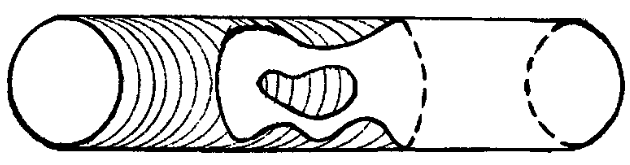
\includegraphics[width=0.8\textwidth]{cobordism-example-1.png}
            \label{fig:cobordism-example-1-png}
        \end{figure}
        In particular, the manifolds in a cobordism
        are \textbf{not} assumed to be connected.
    \end{note}

    \begin{definition}[]
        Consider cobordism classes from $M$ to itself.
        These form a monoid $H_M$. The invertible
        coboridisms in $H_M$ form a group $G_M$.
    \end{definition}

    \begin{definition}[$c_h$]
        Given a diffeomorphism
        $h \colon M \to M'$, define
        $c_h$ as the class of
        $\left( M \times I; M \times 0, M \times 1;
        j, h_1 \right) $ where
        $j (x,0) = x$ and
        $h_1 (x,1) = h(x)$ for $x \in M$.
    \end{definition}
    So a diffeomorphism
    $M \to M'$ gives a cobordism $c_h$ from $M$ to $M'$.

    \begin{theorem}[]
        $c_h c_h' = c_{h'h }$ for any two diffeomorphisms
        $h \colon M \to M'$ and
        $h' \colon M' \to M''$.
    \end{theorem}

    \begin{proof}
        Let
        $W = M \times I \cup_h M' \times I$.
        Let $c_h = \left( M \times I, M \times 0,
        M \times I, ; j_0, j_1 \right) $ and
        $c_{h'} = \left( 
        M' \times I, M' \times 0, M' \times 1,
    j_0', j_1' \right) $.
        So recall that this is formed by taking a tube
        on $M$ and a tube on $M'$ and then gluing an end
        of the tube of $M$ to an end of the tube of $M'$ through
        a twist by the diffeomorphism $h$. Then
        $W$ is still a smooth manifold.
        The resulting cobordism is
        $\left( W, M \times 0, M' \times 1,
        j_0, j_1' \right) $.
        We must show that this is the same, or more
        precisely, that this cobordism is
        \textit{equivalent} to the
        cobordism
        $\left( M \times I,
        M \times 0, M\times 1, j, h_1\right) $ where
        $j(x,0) = x$ and
        $h_1(x,1) = h'h (x)$.
        So we must define a
        diffeomorphism
        $g \colon M \times I \to W$ carrying
        $M \times 0$ to $M \times 0$ and
        $M \times 1$ to $M' \times I$, such that
        for $i = 0,1$, the following triangle commutes
        \begin{equation*}
        \begin{tikzcd}
            M \times 1 \ar[rr, "g|_{M \times 1}"] \ar[dr, "h_1"']
            && M' \times 1 \ar[dl, "j_1'"] \\
                               & M'' &
        \end{tikzcd}
        \end{equation*}
        and
        \begin{equation*}
        \begin{tikzcd}
            M \times 0 \ar[rr, "g|_{M \times 0}"] 
            \ar[dr, "j"] && M \times 0 \ar[dl, "j_0"]\\
                                       & M &
        \end{tikzcd}
        \end{equation*}

        Define
        $g \colon M \times I \to W$ by
        \[
        g(x,t) =
        \begin{cases}
            j_h(x,2t),& t \in \left[ 0 , \frac{1}{2} \right] \\
            j_{h'}\left( h(x), 2t-1 \right) ,& t\in 
            \left[ \frac{1}{2},1 \right] 
        \end{cases}
        \] 
        where
        $j_{h} \colon
        M \times I \to W$ is the inclusion and
        $j_{h'} \colon M' \times I \to W$ is
        the other inclusion given in the
        construction of
        $c_h c_{h'}$.
        Then indeed
        $g|_{M \times 0}$ maps
        into $M \times 0$ and
        $g|_{M \times 1}$ maps into
        $M' \times 1$.
        Furthermore,
        $j_0 \circ g(x,0) = 
        j_0 \circ j_h \left( x,0 \right) 
        = x$ and
        $j_1' \circ g(x,1) = 
        j_1' \circ j_{h'}\left( h(x),1 \right) 
        =j_1'  \left( h(x),1 \right) 
        = h'h(x)
        = h_1(x,1)$, so
        $j_1' \circ g = h_1$.
    \end{proof}

    \subsubsection{Isotopies and Pseudo-Isotopies}

    \begin{definition}[]
        Two diffeomorphisms
        $h_0,h_1 \colon M \to M'$ are
        (smoothly) isotopic if there exists a smooth map
        $f \colon M \times I \to M'$
        such that
        $f_t = f(-,t) \colon M \to M'$ is a diffeomorphism
        for every $t$ and
        $f_0 = h_0$ and $f_1 = h_1$.\\
        Two diffeomorphisms
        $h_0,h_1 \colon M \to M'$ are
        \textit{pseudo-isotopic} if there exists
        a diffeomorphism
        $g \colon M \times I \to M' \times I$ such that
        $g(x,0) = \left( h_0(x), 0 \right) $ and
        $g(x,1) = \left( h_1(x),1 \right) $.
    \end{definition}
    \begin{lemma}[]
        Isotopy and pseudo-isotopiy are equivalence
        relations.
    \end{lemma}

    \begin{theorem}[]
        $c_{h_0} = c_{h_1}$ if and only if
        $h_0$ is pseudo-isotopic to $h_1$.
    \end{theorem}

    \begin{proof}
        Let $g \colon M \times I \to M' \times I$ be a
        pseudo-isotopy between $h_0$ and $h_1$.
        Define
        $h_0^{-1} \times \id \colon M' \times I
        \to M \times I$ by
        \[
            \left( h_0^{-1} \times \id \right) (x,t)
            = \left( h_0^{-1}(x),t \right) .
        \] 
        We claim that
        $\left( h_0^{-1} \times \id \right) \circ g$ 
        is an equivalence 
        between $c_{h_1}$ and $c_{h_0}$.
        Firstly, 
        $\left( h_0^{-1}\times \id \right) 
        \circ g$ is indeed a map
        $M \times I \to M \times I$.
        If we write
        $c_{h_0} = 
        \left( M \times I; M \times 0,
        M \times 1; j_0, k_0 \right) $ and
        $c_{h_1} = \left( M \times I; M \times 0,
        M \times 1; j_0', k_0' \right) $ where
        $j_0(x,0) = x$,
        $j_0'(x,0) = x$ and
        $k_0(x,1) = h_0(x)$ and
        $k_0'(x,1) = h_1(x)$, then firstly,
        $\left( h_0^{-1}\times \id \right) \circ g
        (x,0) = \left( h_0^{-1} \times \id \right) 
        \left( h_0(x),0 \right) 
        = (x,0)$ and
        $\left( h_0^{-1} \times \id \right) \circ
        g(x,1) = \left( h_0^{-1} \times \id \right) 
        \left( h_1(x),1 \right) 
        = \left( h_0^{-1}\circ h_1(x),1 \right)
        \in M \times 1$, and lastly,

        \[
        k_0 \circ \left( h_0^{-1} \times \id \right) \circ g
        (x,1) = 
        k_0 \left( h_0^{-1} \circ h_1(x),1 \right) 
        = h_1(x) = 
        k_0' (x,1) 
        \] 
        and
        \[
        j_0 \circ \left( h_0^{-1} \times \id \right) 
        \circ g(x,0) = 
        j_0 (x,0) = x = 
        j_0' (x,0)
        \] 
        so
        $\left( h_0^{-1} \times \id \right) \circ g$ defines
        an equivalence from
        $c_{h_1}$ to $c_{h_0}$.
    \end{proof}


    \subsubsection{Interlude}

        A different way to define a cobordism is as follows:

        \begin{definition}[]
        A smooth compact $n$-dimensional manifold is
        said to be a cobordism between two $(n-1)$-dimensional
        smooth manifolds $M_L$ and $M_R$ if
        there exist open embeddings
        $M_L \times \mathbb{R} \hookrightarrow M$ and
        $M_R \times \mathbb{R} \hookrightarrow
        M$ such that
        the images of
        $M_R \times [0, \infty)$ and
        $M_L \times (-\infty, 0]$ are closed.
        We denote this by
        $M_L \rightsquigarrow M_R$
        \end{definition}

        \begin{definition}[Gluing cobordisms/composition
            of cobordisms]
            Given cobordisms $M_L \rightsquigarrow M_R =
            N_L \rightsquigarrow N_R$, we can
            form the composite cobordism
             $M \circ N$ as the pullback
             \begin{equation*}
             \begin{tikzcd}
                 M_L \times \mathbb{R}
                 \ar[dr, hookrightarrow]&& M_R \times \mathbb{R}
                 = N_L \times R \ar[dl, hookrightarrow] \ar[dr,
                 hookrightarrow]
                                       && N_R \times \mathbb{R} 
                                       \ar[dl, hookrightarrow]\\
                                       &M \ar[dr, hookrightarrow]&&
                 N\ar[dl, hookrightarrow]&\\
                 &&M \circ N \ar[uu, phantom, "\lrcorner" labl, very
                 near start]&&
             \end{tikzcd}
             \end{equation*}
        \end{definition}


        \begin{definition}[Isomorphism/Equivalence of Cobordisms]
            In this definition, two
            cobordisms
            $M_1 \colon M_L \rightsquigarrow M_R$ and
            $M_2 \colon M_L \rightsquigarrow M_R$ are
            isomorphic/equivalent when there exist maps
            making the following diagram commute:
            \begin{equation*}
            \begin{tikzcd}
                M_L \times R \ar[r, hookrightarrow]
                \ar[d, dash, "\id"']
                & M_1 \ar[d, "f"', "\cong"] & M_R
                \times \mathbb{R} \ar[l, hookrightarrow]
                \ar[d, dash, "\id"] \\
                M_L \times \mathbb{R} \ar[r, hookrightarrow]
                & M_2 & M_R \times 
                \mathbb{R} \ar[l, hookrightarrow]
            \end{tikzcd}
            \end{equation*}
        \end{definition}


        \begin{definition}[Identity cobordism]
            For a smooth compact manifold $M$, the
            identity cobordism of $M$ is the cobordism
            from  $M$ to $M$ given by
            $M \times \mathbb{R}$ where
            we embed
            $M \times \mathbb{R}_{<0} \hookrightarrow
            M \times \mathbb{R}$ 
            and $M \times \mathbb{R}_{>0} 
            \hookrightarrow M \times \mathbb{R}$ by
            the inclusions.
        \end{definition}

        \begin{definition}[Trivial cobordism]
            A cobordism is trivial if it is equivalent to
            an identity cobordism.
        \end{definition}


        \subsection{Elementary Cobordisms}

        \begin{definition}[Gradient-like vector fields for
            Morse functions]
            Let $f$ be a Morse function for the
            triad 
            $\left( W^{n}; V, V' \right) $. A vector field
            $\xi$ on $W^{n}$ is a \textit{gradient-like
            vector field for $f$} if
            \begin{enumerate}
                \item $\xi (f) >0$ throughout the complement
                    of the set of critical points of $f$
                \item Given any critical point $p$ of $f$,
                    there are coordinates
                    $\left( x,y \right) =
                    \left( x_1, \ldots, x_{\lambda},
                    x_{\lambda +1}, \ldots,
                x_n\right) $ in a neighborhood $U$ of $p$ 
                such that
                $f = f(p) - \left| x \right|^2 +
                \left| y \right|^2$ and
                $\xi$ has coordinates
                $\left( -x_1, \ldots, -x_{\lambda},
                x_{\lambda +1}, \ldots,
            x_n\right) $ throughout $U$.
            \end{enumerate}
        \end{definition}

        \begin{remark}[]
            We identify the triad
            $\left( W; V_0, V_1 \right) $ with the
            cobordism
            $\left( W; V_0, V_1 ; i_0, i_1 \right) $ where
            $i_0 \colon V_0 \to V_0 $ and
            $i_1 \colon V_1 \to V_1$ are the identity maps.
        \end{remark}

        \begin{definition}[Product cobordism]
            A triad $\left( W; V_0,V_1 \right)  $ is said
            to be a \textit{product cobordism} if it
            is diffeomorphic to the trivial cobordism
            $\left( V_0 \times \left[ 0,1 \right] ; V_0
            \times 0, V_0 \times 1\right) $.
        \end{definition}

        \begin{theorem}[Identifying product/trivial cobordisms]
            If the Morse number $\mu$ of a triad
            $\left( W; V_0, V_1 \right) $ is zero, then
            $\left( W; V_0,V_1 \right) $ is a product cobordism.
        \end{theorem}

        \begin{theorem}[Collar Neighborhood Theorem]
            Let $W$ be a compact smooth manifold with
            boundary. There exists a neighborhood of
            $\partial W$ (called a collar neighborhood)
            diffeomorphic to 
            $\partial W \times [0,1)$.
        \end{theorem}

        \begin{definition}[Two-sided]
            A connected, closed submanifold
            $M^{n-1} \subset 
            W^{n} - \partial W^{n}$ is said to be
            \textit{two-sided} if some neighborhood
            of $M^{n-1}$ on $W^{n}$ is cut
            into two components when $M^{n-1}$ is deleted.
        \end{definition}


        \begin{theorem}[The Bicollaring Theorem]
            Suppose that every component of
            a smooth submanifold $M$ of $W$ is
            compact and two-sided. Then there
            exists a "bicollar" neighborhood of
            $M$ in $W$ diffeomorphic to
            $M \times (-1,1)$ in such a way that
            $M$ corresponds to
            $M \times 0$.
        \end{theorem}








        \newpage

        \subsubsection{Problems}

    \begin{problem}[Invertible cobordisms and boundaries of
        compact manifolds]
        Let 
        $W_0 \colon M_0 \rightsquigarrow \varnothing $ and
        $W_1 \colon M_1 \rightsquigarrow \varnothing$ be
        two compact $d$-dimensional smooth cobordisms
        from compact $\left( d-1 \right) $-dimensional
        smooth manifolds $M_0$ and $M_1$ to the
        empty manifold, viewed as a 
        $\left( d-1 \right) $-manifold. In other words,
        we have a smooth embedding
        $M_i \times \mathbb{R} \hookrightarrow W_i$ satisfying
        that $M_i \times (-\infty, 0]$ is
        closed, and such that
        their complement 
        $W_i - \left( M_i \times \mathbb{R} \right) $ 
        is compact. We define
        $\Int \left( W_i \right) $ to
        be the complement of the image of
        $M_i \times (- \infty, t]$ for some $t \in \mathbb{R}$ 
        (and hence any $t \in \mathbb{R}$), and observe
        that $\Int \left( W_i \right) $ is again a
        smooth manifold, being an open subset of $W_i$.
        \begin{enumerate}
            \item Assume that in the situation of the
                above, $\Int (W_0)$ is diffeomorphic
                to $\Int \left( W_1 \right) $. Show that
                $M_0$ and $M_1$ are invertibly cobordant,
                i.e., there exists a cobordism
                $M_0 \rightsquigarrow M_1$ which is invertible
                in the category $\Cob_d$.
            \item Let $W$ be a smooth, open
                (i.e., non-compact) $d$-manifold. We define
                a compact closure of $W$ to be a compact
                cobordism $W' \colon
                M \rightsquigarrow \varnothing$ such that
                $W$ is diffeomorphic to 
                $\Int (W')$. Assume that $W$ admits
                a comapct closure $W' \colon M \rightsquigarrow
                \varnothing$. Show that the set of
                compact closures of $W$ up to isomorphism
                of their interiors is in bijection with the
                set of invertible cobordisms over $M$.
        \end{enumerate}
    \end{problem}

    \begin{proof}
        (1)

         Saying that
        $M_0 \rightsquigarrow M_1$ is invertible
        in $\Cob_d$ is precisely saying that
        there exists a cobordism
        $M_1 \rightsquigarrow M_0$ such that the
        composite cobordism
        $M_0 \rightsquigarrow M_1\rightsquigarrow M_0$ 
        is equivalent to the trivial cobordism
        $M_0 \rightsquigarrow M_0$. We
        will do this using the usual definition
        of cobordisms with boundaries. Then
        the problem is equivalently to show that
        we can find coborisms
        $M_0 \rightsquigarrow M_1\rightsquigarrow M_0$ 
        such that
        the composite
        is a product cobordism - i.e., has Morse number
        $0$.
        In this case, we are dealing with closed
        compact manifolds
        $W_0, W_1$ such that
        $\partial W_0 \cong M_0$ and
        $\partial W_1 \cong M_1$. Furthermore,
        the boundaries have closed collar
        neighborhoods
        $\partial W_i \times I$, and removing some open/usual collar
        neighborhoods of these boundaries $\partial W_i \times 
        [0,1)$
        leaves us with compact spaces which are, by
        assumption, diffeomorphic.
        Now, take
        the cobordism $W_0$ and choose
        a collar neighborhood of $\partial W_0 $:
        $M_0 \times [0,1]$, where
        $M_0$ is identified with $M_0 \times 0$ in $W_0$.
        By assumption, there is a diffeomorphism
        $W_0 - \left( M_0 \times [0,1] \right) 
        \cong W_1 - \left( M_1 \times [0,1] \right) $.
        Now, the diffeomorphism
        extends to the closure of the interiors
        which is also $M_i$ since the collar is a cylinder, so
        we obtain a diffeomorphism
        $h \colon M_0 \times 1 \cong M_1 \times 1$. Without
        loss of generality, we can reparametrize, to get the
        diffeomorphism
        $h \colon M_0 \times 1 \to M_1 \times 0$ since
        the boundaries of the interiors must map to each other.
        Now we can glue the collars by gluing the cobordisms
        they represent using theorem 1.4 in Milnor's book
        on h-cobordisms to get a cobordism
        $c_h $ which is the manifold
        $M_0 \times [0,1] \cup_h M_1 \times [0,1]$.
        This indeed now gives a cobordism
        $M_0 \rightsquigarrow M_1$. We can likewise
        obtain the cobordism
        $M_1  \rightsquigarrow M_0 $ which is also obtained
        by gluing
        $M_1 \times [0,1]$ with $M_0\times  [0,1]$ along
        $M_1 \times 1$ and $M_0 \times 0$. Denote this
        cobordism by $c_{h'}$.
        We claim that $c_{h} c_{h'} = \id_{M_0}$. That is, that
        $c_{h} c_{h'}$ is a product cobordism/trivial cobordism
        of $M_0$. One way to see this is
        by using theorem 1.6 in Milnor's book on $h$-cobordisms
        which says that
        $c_{h} c_{h'} = c_{h' h} = c_{\id_{M_0}}$ which indeed
        is the trivial cobordism.
        Alternatively, each collar neighborhood has no
        critical values, so 
        $c_h$ and $c_{h'}$ both have Morse number $0$, and
        then corollary 3.8 in Milnor's book on
        $h$-cobordisms gives that
        $c_h c_{h'}$ also has Morse number $0$, hence
        is trivial by theorem 3.4 in the same book.
    \end{proof}



    \newpage


    \subsection{Morse Functions}

    The goal is to be able to factor cobordisms into
    compositions of simpler cobordisms.

    \begin{definition}[Critical points and non-degenerate
        critical points]
        Let $W$ be a smooth manifold and
        $f \colon W \to \mathbb{R}$ a smooth function.
        A point $p \in W$ is a critical point of
        $f$ if, in some coordinate system,
        \[
        \frac{\partial f}{\partial x^{1}}|_{p} = 
        \frac{\partial f}{\partial x^2}|_{p} = \ldots 
        = \frac{\partial f}{\partial x^{n}}|_p = 0.
        \] 
        Such a point is called a non-degenerate critical
        point if $\det \left( H(f)_p \right) 
        = \det \left( \frac{\partial^2 f}{\partial x^{i}
        \partial x^{j}}|_p \right) \neq 0$
    \end{definition}

    \begin{lemma}[Morse Lemma]\label{Morse-Lemma}
        If $p$ is a non-degenerate critical point of
        $f$, then in some coordiante system about $p$,
        \[
        f\left( x_1, \ldots, x_n \right) =
        c - x_1^2 - \ldots - x_{\lambda}^2 +
        x_{\lambda+1}^2 + \ldots + x_{n}^2
        \] 
        for $\lambda$ between $0$ and $n$ and
        $c$ some constant.
    \end{lemma}

   \begin{definition}[Index of a critical point]
       The $\lambda$ from the Morse Lemma (Lemma~\ref{Morse-Lemma})
       is called the index of the critical point $p$.
   \end{definition} 

   \begin{definition}[Morse Function]
       A \textit{Morse function} on a smooth
       manifold triad
       $\left( W; V_0,V_1 \right) $ is a smooth
       function $f \colon W \to \left[ a,b \right] $ 
       such that
       \begin{enumerate}
           \item $f^{-1}(a) = V_0$ and $f^{-1}(b) = V_1$ 
           \item All the critical points of $f$ are
               interior (lie in $W - \partial W$ ) and
               are non-degenerate.
       \end{enumerate}
   \end{definition}

   \begin{corollary}
       A Morse function has only finitely many zeros.
   \end{corollary}

   \begin{proof}
       Suppose we have a Morse function
       $f \colon W \to \left[ a,b \right] $ and
       suppose that  $p$ is
       a critical point. By definition, it is non-degenerate
       since $f$ is a Morse function, so by the
       Morse Lemma, in some neighborhood of
        $p$, $f$ takes the form
       \[
       f\left( x_1, \ldots, x_n \right) 
       = c - x_1^2 - \ldots - x_{\lambda}^2 +
       x_{\lambda+1}^2 + \ldots+ x_{n}^2
       \] 
       so in particular,
       $\frac{\partial f}{\partial x^{i}} 
       \left( x_1,\ldots,x_n \right) 
       = -2x_i$ in this neighborhood for all $i$.
       Hence $\left( x_1, \ldots, x_n \right) 
       = \left( 0,\ldots,0 \right) $ in this neighborhood
       is the only critical point (in particular,
       in local coordinates, $p = \left( 0,\ldots,0 \right) $ ).
       This shows that critical points of a Morse
       function are isolated. Since
       the manifold of a smooth manifold triad is, in particular,
       compact, there are only finitely many critical points
       since a collection of isolated points in a compact
       space is finite.
   \end{proof}

   \begin{definition}[Morse number $\mu$]
       The \textit{Morse number} $\mu$ of $\left( W;
       V_0, V_1\right) $ is the minimum over all
       Morse functions $f$ on $\left( W;V_0,V_1 \right)$
       of the number of critical
       points of $f$.
   \end{definition}

   \begin{theorem}[Existence of
       Morse functions]\label{Existence-of-Morse-functions}
       Every smooth manifold triad
       $\left( W;V_0,V_1 \right) $ possesses
       a Morse function.
   \end{theorem}

   To prove the existence theorem of Morse functions, 
   we need the following lemmas:

   \begin{lemma}[]
       There exists a smooth function
       $f \colon W \to \left[ 0,1 \right] $ with
       $f^{-1}(0) = V_0, f^{-1}(1) = V_1$, such that
       $f$ has no critical points in a neighborhood
       of the boundary of $W$.
   \end{lemma}

   \begin{lemma}[M. Morse]
       If $f$ is a $C^2$ mapping of an open subset
       $U \subset R^{n}$ to the real line, then,
       for almost all linear mappings
       $L \colon R^{n} \to R$, the function
       $f + L$ has only nondegenerate critical
       points.
   \end{lemma}

   \begin{proof}
       The idea of the proof is
       to consider the manifold
       $U \times \Hom_{\mathbb{R}} \left( \mathbb{R}^{n},
       \mathbb{R} \right) $ the its submanifold
       $M = 
       \left\{ \left( x,L \right)  \mid 
       d\left( f(x) + L(x) \right) = 0\right\} $.
       Then $x\mapsto \left( x,-df(x) \right) $ is
       a diffeomorphism $U \cong M$. Composing with
       a projection $\pi \colon M \to \Hom\left( \mathbb{R}^{n},
       \mathbb{R}\right) $ sending
       $\left( x,L \right) \mapsto L$, one sees that
       $\pi$ is critical at $\left( x,L \right) \in M
       \cong U$ 
       if and only if
       $d\pi = - \frac{\partial^2 f}{\partial x_i 
       \partial x_j}$ is singular. That is, 
       $f + L$ has a degenerate critical point
   \end{proof}
        

\printbibliography
\end{document}
